% Especificaciones del tamaño de letra, tamaño de hoja, márgenes, librerias, etc.
\documentclass[letterpaper]{article}
\usepackage[english]{babel}
\usepackage[utf8]{inputenc}
\usepackage[T1]{fontenc}
\usepackage{mathrsfs}
\usepackage{amsmath}
\usepackage{graphicx}
\usepackage[justification=centering]{caption}
\usepackage{subcaption}
\usepackage[hidelinks]{hyperref}
\usepackage{url}
\usepackage{amssymb}
\usepackage{float}
\usepackage[framed, numbered]{matlab-prettifier}
\usepackage{lipsum}
\usepackage{multicol}
\usepackage{fancyhdr}
%\usepackage[framed, numbered, autolinebreaks, useliterate]{mcode}
\usepackage[margin=1in]{geometry}
\usepackage{titlesec}
\titlelabel{\thetitle.\quad}
\titleformat*{\section}{\normalsize\centering}
\titleformat*{\subsection}{\normalsize\centering}
\renewcommand{\thesection}{\Roman{section}}
\renewcommand{\baselinestretch}{1.3}

\pagestyle{fancy}
\fancyhf{}
\rhead{C. A. VÁSQUEZ}
\lhead{ON COMPOSITE MATERIALS}
\rfoot{\thepage}

% Enlace Bibliografía
\usepackage{csquotes}
\usepackage[backend=biber, sorting=none]{biblatex}
\addbibresource{referencias.bib}

% Titulo, autores, fecha.
\title{\textbf{ON THE SELECTION OF MATERIALS}}
\author{C. A. Vásquez\\
\footnotesize {\textit{UABC, Engineering Department, Mexicali, México}}\\
\footnotesize \texttt{a1155057@uabc.edu.mx}}
\date{}
% Inicio del documento
\begin{document}
\maketitle

\begin{abstract}
	Whether we want to have the most reliable aircraft or the cheapest way to design a product, one thing is for certain, the material we are going to use will determine most of these factors. It is important to keep in mind all the requirements the product in question will need to accomplish, and a method which is useful when designing a product is the selection of materials. The material chosen will dictate the properties, reliability and cost of the product as a whole, therefore it is a field of study which is worth knowing, as it will provide the information needed to make the right decisions.
\end{abstract}
	{\bf Keywords---} materials, stiffness, composites

\begin{multicols}{2}
	\section{INTRODUCTION}
	Whenever the design of a product takes place, several decisions have to be made for the optimal production of the product. When it comes to real-life decision-making, it frequently requires that a compromise between conflicting objectives is made. For example, a design might require a material which is highly reliable and strong, but also lightweight and to top it off, it's needed to be cheap. As anyone can imagine, finding such material isn't within our graps. Thus, decisions shall be made in order to accomplish most of the requirements if possible.

	Depending on the product and overall application of the material is what will determine the material chosen. It may be needed a strong material for safety reasons, in this case if we prioritize safety over cost it's more likely that the product will be expensive but secure. This is where design enters an ethical realm instead of the usual physical realm. Even if this is the case, the objective of choosing a material is to optimise a number of metrics of performance in the product in which it will be used. Some common metrics considered are cost, mass, volume, power-to-weight ratio and energy density. Although optimising a metric usually comes with drawbacks for other metrics, and active research field is the possibility of multi-criteria material selection in order to optimise more many metrics at once. \supercite{pasu04}

	\section{SELECTION AND ITS MOTIVATION}
	Selecting a material is primarly about an awareness and understanding of: 
	\begin{enumerate}
		\item What materials are available.
		\item What processes for shaping these materials are available and how this affects their properties.
		\item The cost of the materials in relation to each other, their processing and their properties.
	\end{enumerate}
	Even if there are thousands of possible materials that the design engineer can choose from, we can group them into a number of broad categories in order to facilitate the discrimination of the materials by basic properties, as seen in figure 1.
	\begin{figure}[H]
		\centering
		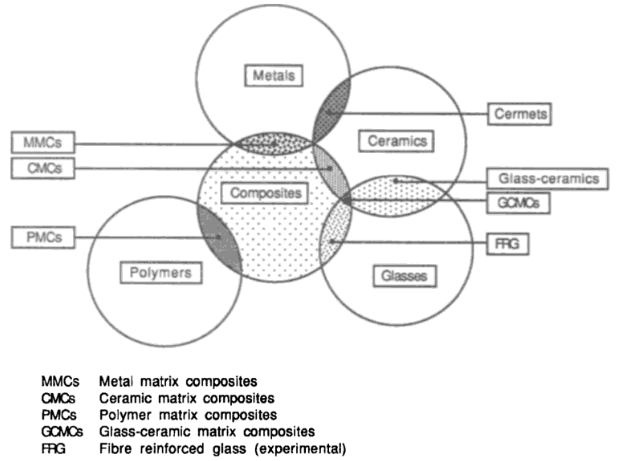
\includegraphics[width=0.5\textwidth]{family.png}
		\caption{The engineering materials family}
	\end{figure}

	There are two main scenarios in which materials selection is needed:
	\begin{enumerate}
		\item Development of a new product.
		\item Improvement of an existing product.
	\end{enumerate}
	In the scope of this paper we shall only consider the development of a new product as it is the more general scenario, from it follows scenario 2.
	
	The general product design process is summarized in figure 2, the three main stages of the design process are as follow:

	\begin{enumerate}
		\item Conceptual design: possible designs are produced as block diagrams representing the main components with some idea of layout.
		\item Embodiment design: this stage involves refining the conceptual designs so that a version exists suitable for marketing and manufacturing teams to visualize the product, usually from computer-generated images. Overall dimensions and shape are emerging at this stage, as are the generic classes of material and processing techniques to be used.
		\item Detailed design: at which stage the preferred layout design is fully dimensioned. Materials and process selection is also now refined to approach a specification.
	\end{enumerate}

	Something important to be noted is that design is an iterative process. Once an item goes into production, the results need to be analysed and the design and manufacturing stages can be reviewed, opening the possibility to make improvements to the product. \supercite{charles97}
	\section{ANALYSIS OF MATERIAL PERFORMANCE REQUIREMENTS}
	When the selection of the material is needed several of its properties are to be measured in order to make the proper selection, aswell as their perfomance under specific conditions (which will depend on the product and its purpose).

	The material perfomance requirements can be divided into five broad categories, namely functional requirements processability requirements, cost, reliability and resistance to services conditions.
	
	The \textbf{functional requirements} are directly related to the required characteristics of the part or product. For example if the part carries a uniaxial tensile load, the yield strength of a candidate material can be directly related to the load-carrying capacity of the product. For these kinds of requirements, an Ashby chart is very useful as it details the distinct properties of a material or group of materials. Some examples of these include the modulus-density charte (shown in figure 3), the strength-density chart, the fracture toughness-density chart, and many more, depending on the properties of interest.\supercite{ashby92}

	The \textbf{processability} of a material is a mesure of its ability to be worked and shaped into a finished part. With reference to a specific manufacturing method, processability can be defined as castability, weldability, machinability, etc. Ductility and hardenability can be relevant if the material is to be deformed or hardened by heat treatment, respectively.
\end{multicols}
\begin{figure}[H]
	\centering
	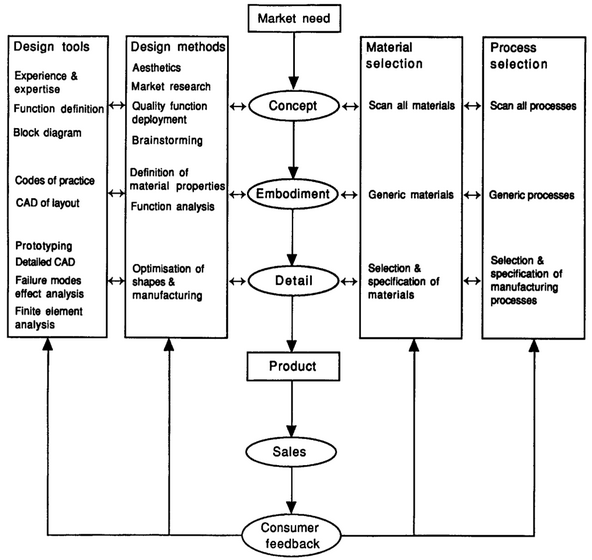
\includegraphics[width=0.7\textwidth]{chart.png}
	\caption{The product design process.}
\end{figure}
\begin{multicols}{2}
	\begin{figure}[H]
		\centering
		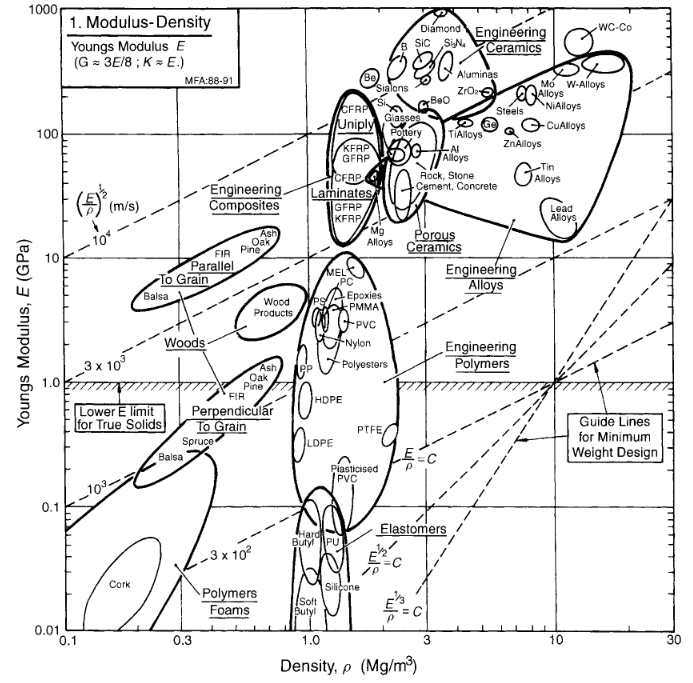
\includegraphics[width=0.5\textwidth]{ashby.png}
		\caption{Modulus-density chart. The heavy envelopes enclose data for a given class of material. The diagonal contours show the longitudinal wave velocity. The guide lines allow selection of materials for minimum weight, deflection-limit, design.}
	\end{figure}
	\textbf{Cost} is usually an important factor in evaluating materials because in many applications there is a cost limit for a material intended to meet the application requirements. When the cost limit is exceeded, the design may need to be changed in order to use less expensive material.

	The \textbf{reliability} of a material can be defined as the probability that it will perform the intended function for the expected life without failure. This is difficult to measure because it is not only dependent upon the material's inherent properties, but it is also greatly affected by its production and processing history. This is often an important selection factor despite its difficulties evaluating it.

	Lastly, the \textbf{environment} in which the product or part will operate plays an important role in determining the material performance requirements (this is also known as the resistance to service conditions).\supercite{kutz02}
	\section{CONCLUSION}
	Although the more technical discussion of the selection of materials was not met in the scope of this paper, it is fair to say that it is one of the most difficult task. Having to look at the huge possibilities of materials that can be used, along with the new generation materials is a complete challente. If we can apply different restrictions (e.g., client specifications, cost, shape, purpose), the selection of material will narrow into small groups. This way, a decision is easier to make and the vast number of possibilities shrinks to a small amount of what it was.
\end{multicols}
%%%%% Bib
\renewcommand\refname{REFERENCES}
\printbibliography

\end{document}
